% !TEX encoding = UTF-8 Unicode

% This is a simple template for a LaTeX document using the "article" class.
% See "book", "report", "letter" for other types of document.
\documentclass[12pt,oneside]{article}
 % use larger type; default would be 10pt


\usepackage[utf8]{inputenc} % set input encoding (not needed with XeLaTeX)

%%% Examples of Article customizations
% These packages are optional, depending whether you want the features they provide.
% See the LaTeX Companion or other references for full information.

%%% PAGE DIMENSIONS
\usepackage{geometry}

 % to change the page dimensions
\geometry{a4paper} % or letterpaper (US) or a5paper or....
%\geometry{margins=2in} % for example, change the margins to 2 inches all round
%\geometry{landscape} % set up the page for landscape
%   read geometry.pdf for detailed page layout information

%\usepackage{graphicx} % support the \includegraphics command and options

% \usepackage[parfill]{parskip} % Activate to begin paragraphs with an empty line rather than an indent

%%% PACKAGES
\usepackage{booktabs} % for much better looking tables
\usepackage{array} % for better arrays (eg matrices) in maths
\usepackage{paralist} % very flexible & customisable lists (eg. enumerate/itemize, etc.)
\usepackage{verbatim} % adds environment for commenting out blocks of text & for better verbatim
\usepackage{subfig} % make it possible to include more than one captioned figure/table in a single float
% These packages are all incorporated in the memoir class to one degree or another...

%%% HEADERS & FOOTERS
%\usepackage{fancyhdr} % This should be set AFTER setting up the page geometry



%%% SECTION TITLE APPEARANCE

 % (See the fntguide.pdf for font help)
% (This matches ConTeXt defaults)

%%% ToC (table of contents) APPEARANCE
%\usepackage[nottoc,notlof,notlot]{tocbibind} % Put the bibliography in the ToC
%\usepackage[titles,subfigure]{tocloft} % Alter the style of the Table of Contents
\usepackage[encapsulated]{CJK} 


\usepackage{setspace}
\usepackage{amsfonts}
\usepackage{amssymb}
\usepackage{amsmath}
\usepackage{amstext}
\usepackage{amscd}
\usepackage{hyperref}
\usepackage{amsthm}
\usepackage{mathtools}
\usepackage{graphicx} 

\newcommand{\e}[0]{\varepsilon}
\newcommand{\norm}[1]{\left|\left|#1\right|\right|}
\newcommand{\ra}[0]{\rightarrow}
\newcommand{\Ra}[0]{\Rightarrow}
\newcommand{\R}[0]{\mathbb{R}}
\newcommand{\Q}[0]{\mathbb{Q}}
\newcommand{\N}[0]{\mathbb{N}}
\newcommand{\D}[0]{\mathbb{D}}
\newcommand{\BF}[0]{\mathbb{F}}
\newcommand{\CN}[0]{\mathcal{N}}
\newcommand{\Z}[0]{\mathbb{Z}}
\newcommand{\C}[0]{\mathbb{C}}
\newcommand{\CE}[0]{\mathcal{E}}
\newcommand{\CM}[0]{\mathcal{M}}
\newcommand{\CA}[0]{\mathcal{A}}
\newcommand{\CP}[0]{\mathcal{P}}
\newcommand{\CT}[0]{\mathcal{T}}
\newcommand{\cond}[4]{\left \{ \begin{array}{ll} #1 & \mbox{#2} \\ #3 & \mbox{#4} \end{array} \right.}
\newcommand{\condd}[6]{\left \{ \begin{array}{ll} #1 & \mbox{#2} \\ #3 & \mbox{#4} \\ #5 & \mbox{#6}\end{array} \right.}
\newcommand{\conddd}[8]{\left \{ \begin{array}{ll} #1 & \mbox{#2} \\ #3 & \mbox{#4} \\ #5 & \mbox{#6} \\ #7 & \mbox{#8} \end{array} \right.}
\newcommand{\lams}[1]{\lambda^*(#1)}
\newcommand{\bs}[0]{\backslash}
\newcommand{\bM}[0]{\overline{\M}}
\newcommand{\bmu}[0]{\overline{\mu}}
\newcommand{\mus}[0]{\mu^*}
\newcommand{\sa}[0]{\sigma \mbox{-algebra}}
\newcommand{\set}[1]{\{ #1\}}
\newcommand{\CB}[0]{\mathcal{B}}
\newcommand{\CG}[0]{\mathcal{G}}
\newcommand{\CF}[0]{\mathcal{F}}
\newcommand{\CU}[0]{\mathcal{U}}
\newcommand{\CL}[0]{\mathcal{L}}
\newcommand{\FA}[0]{\mathfrak{A}}
\newcommand{\BT}[0]{\mathbb{T}}
\newcommand{\BI}[0]{\mathbb{I}}
\newcommand{\BE}[0]{\mathbb{E}}
\newcommand{\eK}[1]{\e\mbox{-Kronecker}(#1)}
\newcommand{\eKG}[0]{\e\mbox{-Kronecker}}
\newcommand{\KL}[2]{\mbox{{\renewcommand*\rmdefault{}\normalfont KL}}(#1 \ || \ #2)}
\newcommand{\JS}[2]{\mbox{{\renewcommand*\rmdefault{}\normalfont JS}}(#1 \ || \ #2)}

\newcommand{\IN}[1]{I_0(#1)}
\newcommand{\ING}[0]{I_0}
\newcommand{\st}[0]{such that }
\newcommand{\CS}[0]{\mathcal{S}}
\newcommand{\CC}[0]{\mathcal{C}}
\newcommand{\tn}[1]{\text{\normalfont #1}}



\newcommand{\bmp}[1]{\overline{M}^+(#1)}
\newcommand{\simplep}[2]{S_{#1}^+(#2)}
\newcommand{\simple}[2]{S_{#1}(#2)}
\newcommand{\sumf}[2]{\sum_{#1 = #2}^\infty}
\newcommand{\bigcapf}[2]{\bigcap_{#1 = #2}^\infty}
\newcommand{\bigcupf}[2]{\bigcup_{#1 = #2}^\infty}
\newcommand{\limf}[1]{\lim_{#1 \ra \infty}}
\newcommand{\seq}[2]{\set{#1_{#2}}_{#2=1}^\infty}
\newcommand{\sg}[1]{\sigma\langle#1\rangle}
\newcommand{\ag}[1]{\langle#1\rangle}
\newcommand{\g}[1]{\langle#1\rangle}
\newcommand{\inte}[0]{\mbox{int}}
\newcommand{\Cl}[0]{\mbox{cl}}
\newcommand{\bd}[0]{\mbox{bd}}
\newcommand{\inv}[1]{{#1}^{-1}}
\newcommand{\Aut}[0]{\mbox{{\renewcommand*\rmdefault{}\normalfont Aut}}}
\newcommand{\Gal}[0]{\mbox{{\renewcommand*\rmdefault{}\normalfont Gal}}}
\newcommand{\Bor}[0]{\mbox{{\renewcommand*\rmdefault{}\normalfont Bor}}}
\newcommand{\Meas}[0]{\mbox{{\renewcommand*\rmdefault{}\normalfont Meas}}}
\newcommand{\ball}[2]{\mbox{{\renewcommand*\rmdefault{}\normalfont B}}_{#1}({#2})}
\newcommand{\supp}[0]{\mbox{{\renewcommand*\rmdefault{}\normalfont supp}}}
\newcommand{\Trig}[0]{\mbox{{\renewcommand*\rmdefault{}\normalfont Trig}}}
\newcommand{\sign}[0]{\mbox{{\renewcommand*\rmdefault{}\normalfont sign}}}
\newcommand{\AP}[0]{\mbox{{\renewcommand*\rmdefault{}\normalfont AP}}}

\newcommand{\ali}[1]{\begin{align*}#1\end{align*}}
\newcommand{\zhongwen}[1]{\begin{CJK}{UTF8}{gbsn}#1\end{CJK}}
\renewcommand{\Bar}[1]{\overline{#1}}
\renewcommand{\Hat}[1]{\widehat{#1}}
\newcommand{\Ga}[0]{\Gamma}
\newcommand{\ga}[0]{\gamma}
\newcommand{\inner}[2]{\left\langle #1, #2 \right\rangle}
\renewcommand{\Tilde}[1]{\widetilde{#1}}


\theoremstyle{plain}
\newtheorem{thm}{Theorem}[subsection]
\newtheorem{lem}[thm]{Lemma}
\newtheorem*{prop}{Proposition}
\newtheorem*{cor}{Corollary}
\newtheorem{defn}[thm]{Definition}
\newtheorem{exmp}[thm]{Example}


\theoremstyle{remark}
\newtheorem*{rem}{Remark}
\newtheorem*{claim}{Claim}
\newtheorem*{note}{Note}
\newtheorem*{sol}{Solution}
\newtheorem*{case}{Case}


%%% END Article customizations

%%% The "real" document content comes below...

\title{Diffusion Models}
\date{} % Activate to display a given date or no date (if empty),
         % otherwise the current date is printed 
\parindent=0pt 
\begin{document}
\onehalfspace

\sloppy
\maketitle
Suppose data $x_0$ follows some unknown distribution $q(x_0)$.\\
Similar to VAE, in diffusion models, we have the latent variables $x_{1:T}$ with the assumption that $x_{0:T}$ form a Markov chain with Gaussian transitions, starting with $x_T \sim \CN(0, I)$,
\ali{ p_\theta(x_{t-1} | x_{t}) = \CN(x_{t-1}; \mu_\theta(x_{t}, t), \Sigma_\theta(x_t, t))}
for $1 \leq t \leq T$ and the likelihood
\ali{p_\theta(x_{0:T}) = p(x_T) \prod_{t=1}^T p_\theta(x_{t-1} | x_{t}).}
This corresponds to the reverse diffusion process described later.\\
Unlike VAE where we approximate the posterior, the posteriors in diffusion models are assumed to follow a Markov chain:
\ali{q(x_{1:T} | x_0) = \prod_{t=1}^T q(x_t | x_{t-1}).}
The conditional probabilities $q(x_t | x_{t-1})$ are Gaussians: 
\ali{q(x_t | x_{t-1}) = \CN(x_t; \sqrt{1-\beta_t} \ x_{t-1}, \beta_t I),}
where $0 < \beta_t < 1$ are constants. The posteriors correspond to the forward diffusion process.\\

{\bf Objective Function}\\

Similar to VAE, taking $x_{1:T}$ as the latent variables, the ELBO is
\ali{\BE_{q(x_0)} \left[ -\log(p_\theta(x_0)) \right] \leq \BE_{q(x_{0:T})} \left[ \log \frac{q(x_{1:T} | x_0)}{p_\theta(x_{0:T})} \right].}
Since 
\ali{&q(x_{1:T} | x_0) = \prod_{t=1}^T q(x_t | x_{t-1}) \\
     &p_\theta(x_{0:T}) = p(x_T) \prod_{t=1}^T p_\theta(x_{t-1} | x_{t}),}
the ELBO expands
\ali{&\BE_{q(x_{0:T})} \left[ \log \frac{q(x_{1:T} | x_0)}{p_\theta(x_{0:T})} \right] \\
    = \ &\BE_{q(x_{0:T})} \left[ -\log p(x_T) + \sum_{t=2}^T \log \frac{q(x_t | x_{t-1})}{p_\theta(x_{t-1} | x_t)} + \log \frac{q(x_1 | x_0)}{p_\theta(x_0 | x_1)} \right] \\
    = \ &\BE_{q(x_{0:T})} \left[ -\log p(x_T) + \sum_{t=2}^T \log \frac{q(x_{t-1} | x_{t}, x_0)}{p_\theta(x_{t-1} | x_t)} \cdot \frac{q(x_t | x_0)}{q(x_{t-1} | x_0)} + \log \frac{q(x_1 | x_0)}{p_\theta(x_0 | x_1)} \right] \\
    = \ &\BE_{q(x_{0:T})} \left[ \log \frac{q(x_T | x_0)}{p(x_T)} + \sum_{t=2}^T \log \frac{q(x_{t-1} | x_{t}, x_0)}{p_\theta(x_{t-1} | x_t)} -  \log p_\theta(x_0 | x_1) \right] \\
    = \ &\BE_{q(x_{0})}  \left[ \KL{q(x_T | x_0)}{p(x_T)} \right]  \\
    &+ \BE_{q(x_{0:T})} \left[ \sum_{t=2}^T \KL{q(x_{t-1} | x_{t}, x_0)}{p_\theta(x_{t-1} | x_t)} \right] \\
    &- \BE_{q(x_0, x_1)} \log p_\theta(x_0 | x_1) \\
    := \ &L_T + \sum_{t=2}^T L_{t-1} + L_0.}
We will revisit the ELBO and see why we further condition on $x_0$ in above equations.\\ 


{\bf Forward Diffusion Process}\\

By reparametrizing, for independent $\e_i \sim \CN(0, I)$ and $\alpha_t = 1 - \beta_t$,
\ali{x_t &= \sqrt{1-\beta_t} \ x_{t-1} + \sqrt{\beta_t} \ \e_{t-1} \\
         &= \sqrt{\alpha_t} \ x_{t-1} + \sqrt{1-\alpha_t} \ \e_{t-1}.}
Also,
\ali{x_{t-1} = \sqrt{\alpha_{t-1}} \ x_{t-2} + \sqrt{1-\alpha_{t-1}} \ \e_{t-2}.}
Hence,
\ali{x_t = \sqrt{\alpha_t \alpha_{t-1}} \ x_{t-2} + \sqrt{\alpha_t - \alpha_t \alpha_{t-1}} \ \e_{t-2} + \sqrt{1-\alpha_t} \ \e_{t-1}.}
Since $\e_{t-2}$ and $\e_{t-1}$ are independent, 
\ali{\sqrt{\alpha_t - \alpha_t \alpha_{t-1}} \ \e_{t-2} + \sqrt{1-\alpha_t} \ \e_{t-1} \sim \CN(0, (1-\alpha_t \alpha_{t-1}) I).}
We reparametrize
\ali{x_t = \sqrt{\alpha_t \alpha_{t-1}} \ x_{t-2} + \sqrt{1-\alpha_t \alpha_{t-1}} \ \tilde{\e}_{t-2}}
for $\tilde{\e}_{t-2} \sim \CN(0, I)$.\\
Continue this way and we have
\ali{x_t = \sqrt{\bar{\alpha}_t} \ x_0 + \sqrt{1 - \bar{\alpha}_t} \ \e \ \ \ (*)}
for $\e \sim \CN(0, I)$ and $\bar{\alpha}_t = \alpha_1...\alpha_t$.\\ 
In other words
\ali{q(x_t | x_0) = \CN(x_t; \sqrt{\bar{\alpha}_t} \ x_0, \sqrt{1 - \bar{\alpha}_t} I).}
Notice that if $\bar{\alpha}_t \ra 0$, then $q(x_t | x_0) \ra \CN(0, I)$. This is desired as we want pure Gaussian noise after the forward diffusion process.\\

{\bf Reverse Diffusion Process}\\

Notice that the conditional probability $q(x_{t-1} | x_t)$ is tractable when conditioning further on $x_0$ using Bayes' rule:
\ali{q(x_{t-1} | x_t, x_0) &= \frac{q(x_t | x_{t-1}, x_0) q(x_{t-1} | x_0)}{q(x_t | x_0)} \\
                           &= \frac{q(x_t | x_{t-1}) q(x_{t-1} | x_0)}{q(x_t | x_0)} \ \ \ \ \ \ \ \text{(Markov Property)}}
Since
\ali{q(x_t | x_{t-1}) &= \CN(x_t; \sqrt{\alpha_t} \ x_{t-1}, \beta_t I) \\
    q(x_{t-1} | x_0)  &= \CN(x_{t-1}; \sqrt{\bar{\alpha}_{t-1}} \ x_0, \sqrt{1 - \bar{\alpha}_{t-1}} I) \\
    q(x_t | x_0) &= \CN(x_t; \sqrt{\bar{\alpha}_t} \ x_0, \sqrt{1 - \bar{\alpha}_t} I),}
we have
\ali{q(x_{t-1} | x_t, x_0) = \CN(x_{t-1}; \tilde{\mu}_t, \tilde{\beta}_t I)}
for 
\ali{\tilde{\mu}_t &= \tilde{\mu}_t(x_t, x_0) = \frac{\sqrt{\alpha_t} (1 - \bar{\alpha}_{t-1})}{1 - \bar{\alpha}_t} x_t + \frac{\sqrt{\bar{\alpha}_{t-1}} (1 - \alpha_t)}{1 - \bar{\alpha}_t} x_0  \\
    \tilde{\beta}_t &= \frac{1 - \bar{\alpha}_{t-1}}{1 - \bar{\alpha}_t} (1- \alpha_t)}
with some constant terms omitted.\\
Because of the parametrization $(*)$,
\ali{\tilde{\mu}_t = \tilde{\mu}_t(x_t, \e) = \frac{1}{\sqrt{\alpha_t}} \left(x_t - \frac{1 - \alpha_t}{\sqrt{1 - \bar{\alpha}_t}} \e \right)}
for $\e \sim \CN(0, I)$.\\

{\bf Objective Function Revisited}\\

Note that we have nothing to optimize in the $L_T$ term and therefore $L_T$ is omitted from the ELBO.\\
For $L_t$ with $1 \leq t < T$, it is the KL-divergence between two Gaussian distributions:
\ali{ q(x_{t-1} | x_t, x_0) &= \CN(x_{t-1}; \tilde{\mu}_t, \tilde{\beta}_t I) \\
p_\theta(x_{t-1} | x_{t}) &= \CN(x_{t-1}; \mu_\theta(x_{t}, t), \Sigma_\theta(x_t, t)).}
Hence, we set $\Sigma_\theta(x_t, t) = \sigma_t^2 I := \tilde{\beta}_t I$ (without learnable parameters).\\
$\mu_\theta(x_t, t)$ should predict 
\ali{\tilde{\mu}_t = \tilde{\mu}_t(x_t, \e) = \frac{1}{\sqrt{\alpha_t}} \left(x_t - \frac{1 - \alpha_t}{\sqrt{1 - \bar{\alpha}_t}} \e \right)}
for some $\e \sim \CN(0, I)$. Therefore we design 
\ali{\mu_\theta(x_t, t) = \frac{1}{\sqrt{\alpha_t}} \left(x_t - \frac{1 - \alpha_t}{\sqrt{1 - \bar{\alpha}_t}} \e_\theta(x_t, t) \right)}
for some neurel network $\e_\theta(x_t, t)$ predicting $\e$. The objective function $L_{t-1}$ is 
\ali{L_{t-1} &= \BE_{q(x_0, x_{t-1}, x_t)} \left[ \KL{q(x_{t-1} | x_{t}, x_0)}{p_\theta(x_{t-1} | x_t)} \right] \\
             &= \BE_{x_0, \e} \left[ \frac{1}{2\sigma_t^2} \norm{\mu_\theta(x_t(x_0, \e), t) - \tilde{\mu}_t(x_t(x_0, \e), \e)}^2 \right] \\
             &= \BE_{x_0, \e} \left[ \frac{\beta_t^2}{2\sigma_t^2\alpha_t(1-\bar{\alpha}_t)} \norm{\e - \e_\theta(x_t(x_0, \e), t)}^2 \right],}
where $x_t(x_0, \e) =  \sqrt{\bar{\alpha}_t} \ x_0 + \sqrt{1 - \bar{\alpha}_t} \ \e$.\\
$L_0$ will be dealt separately according to $p_\theta(x_{0} | x_{1}) = \CN(x_{0}; \mu_\theta(x_{1}, 1), \sigma_1^2 I)$.\\

{\bf Simplified Objective Function}\\

The objective function $L(\theta) = \sum_{t=2}^T L_{t-1}(\theta) + L_0(\theta)$ can be simplified to 
\ali{L_{\text{simple}}(\theta) = \BE_{x_0, \e, t} \left[ \norm{\e - \e_\theta(x_t(x_0, \e), t)}^2 \right].}

The paper proposed following training and sampling algorithms:

\begin{figure}[h]
    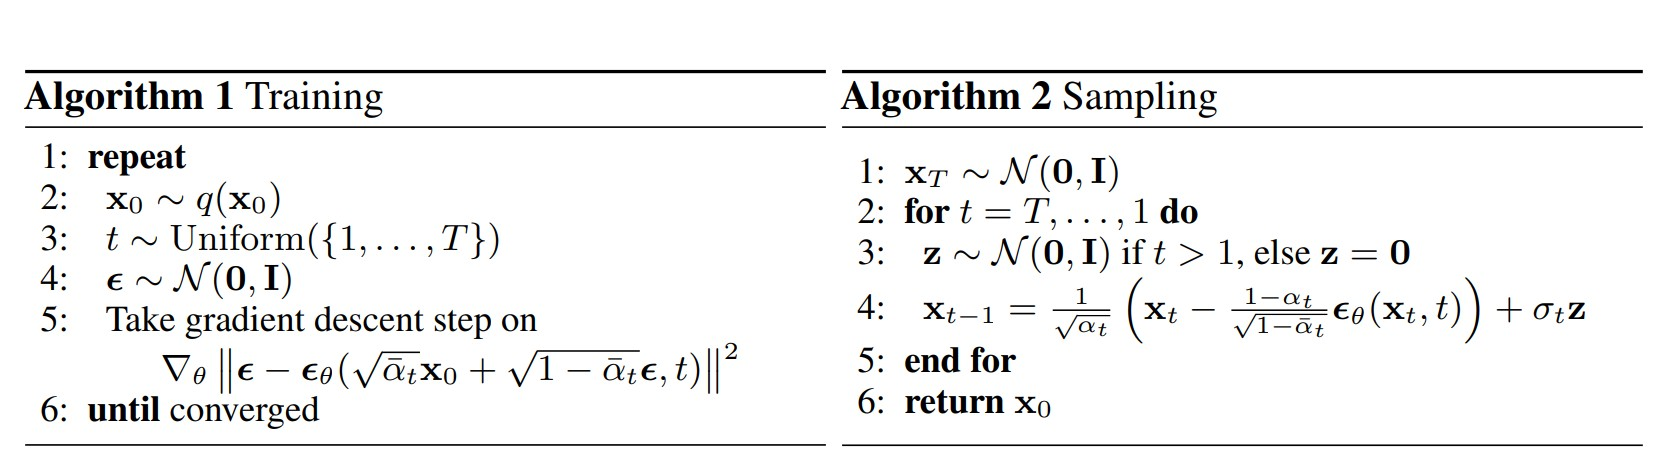
\includegraphics[width=1\linewidth]{diffusion.jpg}
\end{figure}

      






\end{document}